\chapter{Project Implementation}

Initiating the chapter, here project implementation is discussed. The resources required, flowcharts, algorithms as well as proposed layouts have been highlighted here.\\ 

\section{Requirement of Resources}
\begin{itemize}
    \item Software Requirement 
        \begin{enumerate}
            \item OS Requirement:
                \begin{itemize}
                    \item Windows 8/10(Can be used both for Training and at User End)
                    \item Linux(Only at User End)
                \end{itemize}
            \item Training of the model:
                \begin{itemize}
                    \item Python ide(Anaconda Jupyter Notebook/Jupyter Lab)
                    \item Dataset for Training
                \end{itemize} 
            \item Web Application
        \end{enumerate}
    \item Hardware Requirement
        \begin{enumerate}
            \item Basic Hardware for Training Purpose:
                \begin{itemize}
                    \item RAM : 8 GB
                    \item ROM : 2 GB
                    \item Processor : i5 Processor
                \end{itemize}
        \end{enumerate}
    \end{itemize}
    
%%%%%%%%%%%%%%%%%%%%%%%%%%%%%%%%%%%%%%%%%%%%%%%%%%%%%%%%%%%%%%%%%%%%%%%%%%%%%%%%%%%%%%%%%%%%%%%%%%%%%%%%%%%%%%%%%%%%%%%%%%%%%%%%%%%%%%%%%%%%%%%%%%%%%%%%%%%%%%%%%%%%%%%%%%%%%%%%%%%%%%%%%%%%%%%%%%%%%%%%%%%%%%%%%%%%%%%%%%%%%%%%%%%%%%%%%%%%%

\section{Development of the Detection model}
This section explains about the Detection model and it's training. The model developed is the backend of this project, as it handles the core function of determining whether the MRI image present has tumour or not.
\subsection{Algorithm}
Step 1 : Import the libraries.\\ 
Step 2 : Import the dataset.\\ 
Step 3 : Define Label Classes.\\ 
Step 4 : Append data into training set\\ 
Step 5 : Shuffle the training data.\\
Step 6 : Splitting data into train, test, and validation.\\
Step 7 : Import pre-trained model.\\ 
Step 8 : Add your training layers on top of imported model.\\
Step 9 : Compile the model.\\ 
Step 10 : Define Callbacks.\\ 
Step 11 : Train Model.\\ 
Step 12 : Defining Model Layers.\\ 
Step 13 : Plotting the accuracy and loss graphs.\\ 
Step 14 : Evaluating the Model using classification report, manual and automated testing.
\subsection{Flowchart}
The flowchart below describes the process as to how the detection model is developed.
\begin{figure}[H]
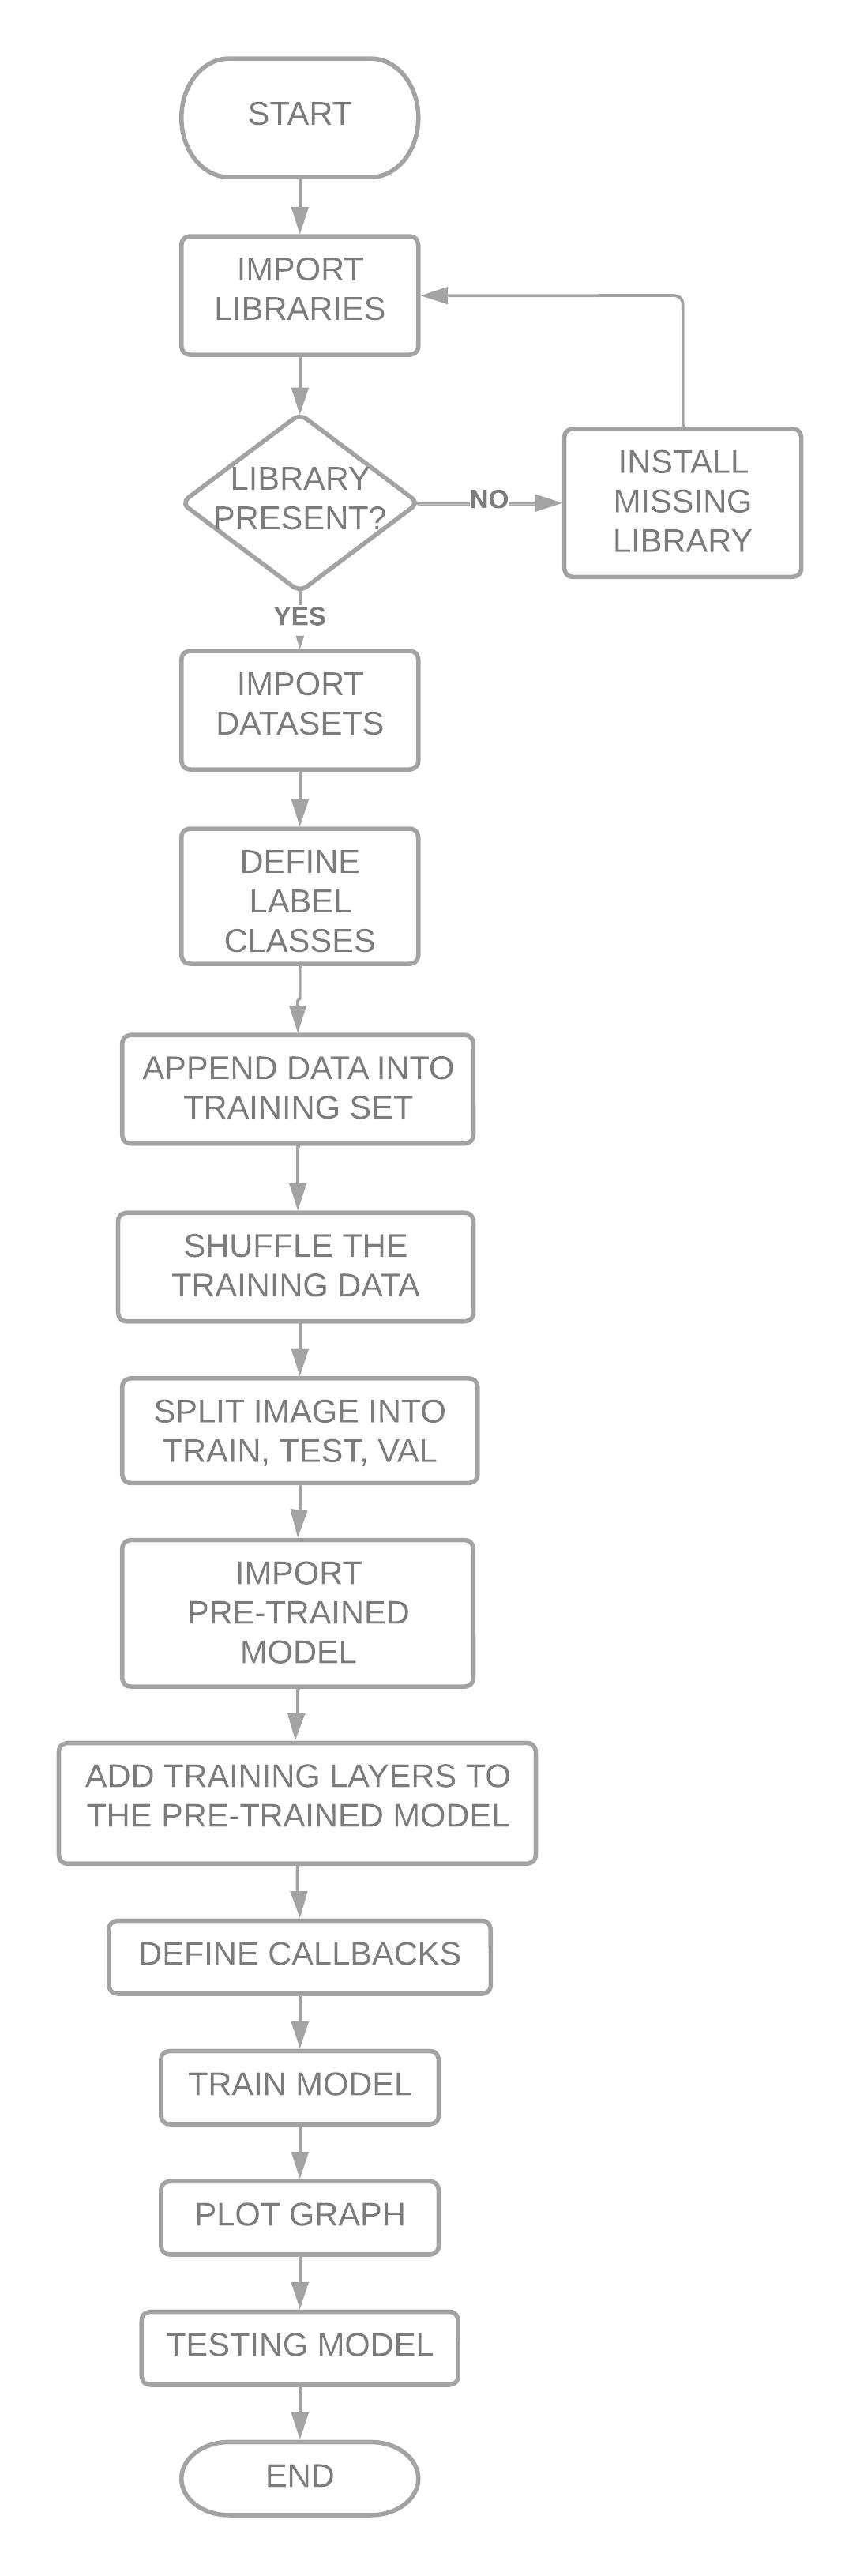
\includegraphics[scale=0.2]{Photos/phase2_model_flowchart.png}
\caption{Model Training Flowchart} \label{fig:Model Summary}
\end{figure}
\subsection{Transfer Learning} \label{subsection:transfer_learning}
Transfer learning is a machine learning concept where a pre-trained model is reused or retrained as the base layer for a model on a new task. In simple words, an already trained model on one task or one problem statement is repurposed for a second, related task. This acts as an optimization that allows rapid progress when modelling the second task is taking place. As observed in figure \ref{fig:transfer_learning} it can be seen that the training layers from Task 1 are transferred as base layers to the task 2, thereby reducing training time, increasing optimization time.
\begin{figure}[H]
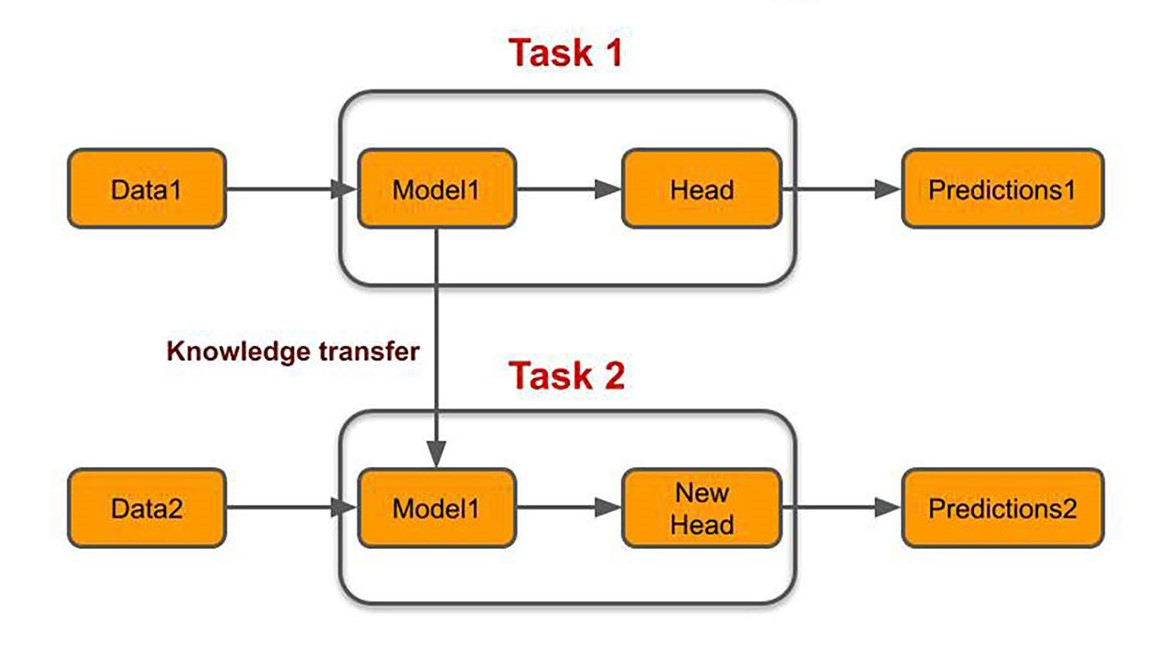
\includegraphics[scale=0.4]{Photos/transfer_learning.jpg}
\caption{Transfer Learning} \label{fig:transfer_learning}
\end{figure}

\subsection{Defining the Model}
A transfer learning based model was used for the project. It is one of the the easiest way to build a model for machine learning applications. As explained in section \ref{subsection:transfer_learning}, already trained model on one task or one problem statement is repurposed for a second, related task. To define the model following libraries must be imported, these libraries are a sub class of "keras.layers" :
\begin{itemize}
    \item Sequential : It is used to initialize the neural network.
    \item Convolution2D : This layer deals with creating a convolutional network that will deal with the MRI images.
    \item MaxPooling2D : This layer adds the pooling layers.
    \item Flatten : This layer converts the pooled feature map to a single column. This is passed to the fully connected layer.
    \item Dense : Dense layer will add this fully connected layer to the neural network.
    \item Dropout : Dropout is a technique used to prevent a model from overfitting.
    \item BatchNormalization : It is a technique for training very deep neural networks that standardizes the inputs to a layer for each mini-batch.
\end{itemize}
%\begin{figure}[H]
%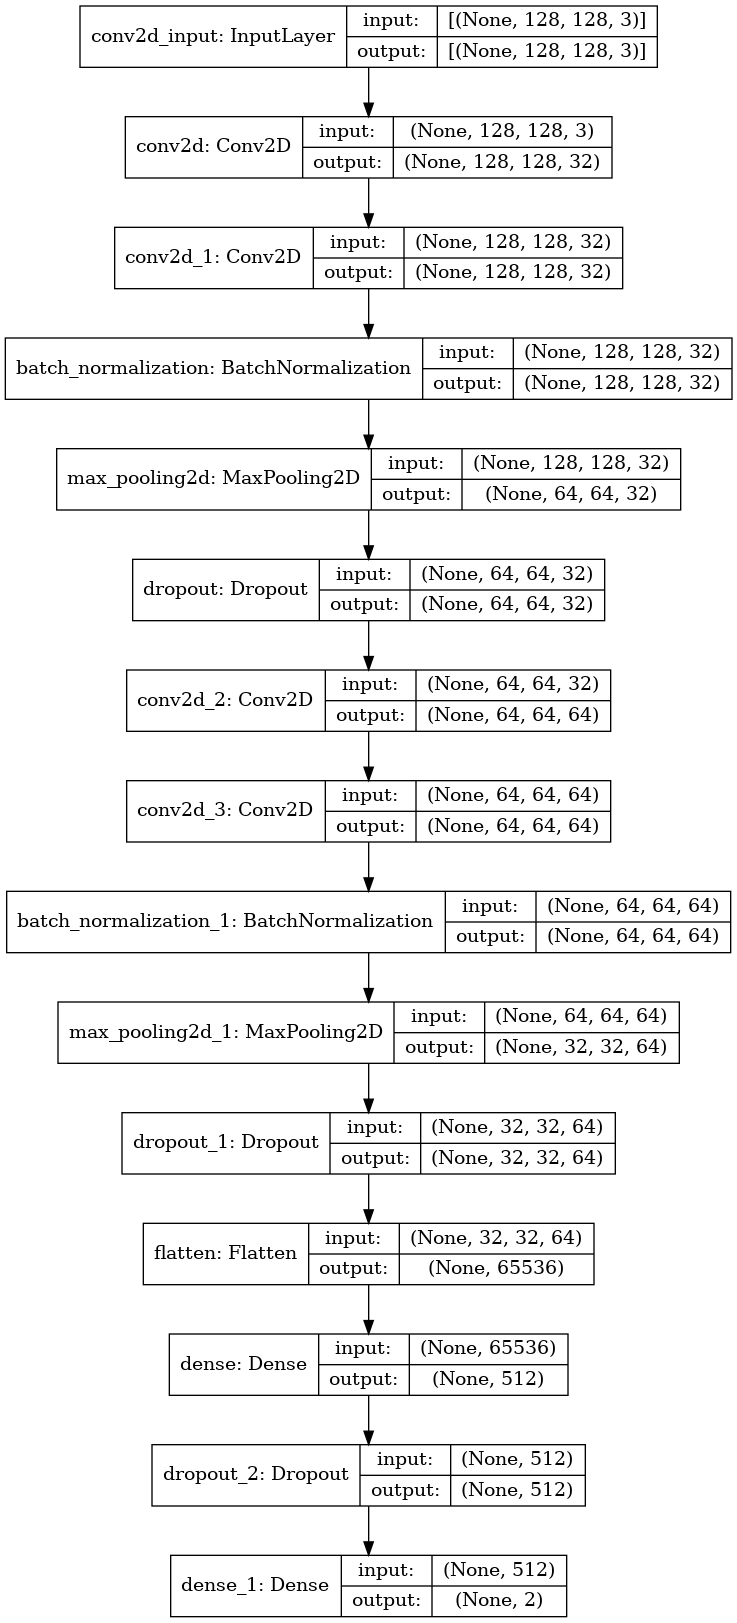
\includegraphics[scale=0.34]{Photos/model_plot.png}
%\caption{Model Summary} \label{fig:model_plot}
%\end{figure}

%%%%%%%%%%%%%%%%%%%%%%%%%%%%%%%%%%%%%%%%%%%%%%%%%%%%%%%%%%%%%%%%%%%%%%%%%%%%%%%%%%%%%%%%%%%%%%%%%%%%%%%%%%%%%%%%%%%%%%%%%%%%%%%%%%%%%%%%%%%%%%%%%%%%%%%%%%%%%%%%%%%%%%%%%%%%%%%%%%%%%%%%%%%%%%%%%%%%%%%%%%%%%%%%%%%%%%%%%%%%%%%%%%%%%%%%%%%%%

\section{Proposed Web Application}
This section explains about the Proposed Web Application. In this section detailed Algorithm is shown, as well as gives an insight on Local Server Deployement and Logs.

\subsection{Welcome Page}
Step 1 : Complete Web application runs on the local host web page in your browser.\\
Step 2 : Video division and basic information is displayed on this page.\\
Step 3 : Top left corner of the web application has option button and drop down menu access which consists of the different routes for the web application.\\
Step 4 : You can click on various routes to get the particular page displayed.

\subsection{Information Page}
Step 1 : Here you find all the basic and medical related info for the Brain Tumours.\\
Step 2 : Scroll down to get additional information for diagnosis, traditional methods and the web application method.\\
Step 3 : Interactivity buttons are added in between to display information about the various tumours and treatment methods.

\subsection{Algorithm}
Step 1 : Web-App is running on Streamlit framework.\\
Step 2 : User inputs the image.
Step 3 : If any other file other than allowed image extension, system logs message as "Enter valid file type only".\\
Step 4 : If input file in accordance with allowed image extension, move to step 5.\\
Step 5 : Input image is passed onto the preexisting Knowledge Base (Detection Model).\\
Step 6 : If tumour is detected, the system further gives an inference between whether the tumour is of : meningioma, pituitary or glioma. Needed output will be printed along with the confidence score.\\
Step 7 : If tumour is not detected, the system returns output as "Tumour Not Detected".

\subsection{Backend Results}
Result : This is the result section where in it shows all the result in the form of confusion matrix, classification report which are respectively explained in the web application's particular route.

\subsection{Team Information Page}
Step 1 : This page consists of the information of our developing team.\\
